\documentclass{article}
\usepackage[utf8]{inputenc}
\usepackage{graphicx}

\title{Rhythms, Sleep, and Dreams}
\author{MCB C61 with Professor David Presti \\ \\ Benjamin Lee}
% \date{8 March 2018}

\begin{document}

\maketitle

\textbf{Key Concepts:}
\begin{itemize}
    \item Sleep 
    \item Circadian rhythms
    \item Melatonin
    \item Circ-annual rhythms and bird migration
    \item Free-running rhythm
    \item Suprachiasmatic nucleus (SCN)
    \item PER, molecular mechanism of circadian clock
    \item Retinal-hypothalamic pathway
    \item Melanopsin 
    \item Jet lag
    \item Human sleep, NREM, REM, stages
    \item Progression of sleep stages
    \item REM sleep and dreams
    \item Acetylcholine and REM
    \item Lucid Dreaming, dream yoga
    \item Sleep disorders: insomnia, apnea, narcolepsy, REM-behavior, sleep paralysis, sleepwalking
    \item Chronic sleep deprivation
    \item Sleep and learning, memory, consolidation
\end{itemize}

\newpage
\section{Sleep}
Periods of inactivity and reduced alertness in many animals is known as \textit{sleep} 

\begin{itemize}
    \item Amount of time spent asleep varies across different species of animal
    \item Sleep times of animals in a 24 hour day: bat, 19; mouse and rat, 12; rabbit, 9; cow and elephant 4
    \item Humans typically sleep 8 hours, a third of our day and lifetime!
    \item If we live 90 years, 30 of those years are spent sleeping (263,000 hours) 
    \item Desire for sleep becomes overwhelming if sleep deprivation and tiredness persists
\end{itemize}

\subsection{Circadian Rhythms}
The regular cycle of sleep and wakefulness in our lives is an example of a biological rhythm
\begin{itemize}
    \item Sleep and wakefulness follow a circadian pattern (Latin \textit{circa} = about, \textit{dies} = day) 
    \item Has a 24 hour periodicity
    \item Other examples of circadian rhythms are body temperature variations and synthesis of cortisol and other glucocorticoids by the adrenal gland
    \item  \textbf{Melatonin:} made by many organisms including bacteria, fungi, and plants as well as animal, serves as a protective antioxidant functions
    \item synthesized in a circadian rhythm from serotonin in pineal gland in vertebrate animals and plays an important role in the \textbf{sleep-wake cycle}
\end{itemize}

Circadian rhythms are found in other organisms as well, such as plants, fungi, and single-celled creatures. Some think that it is the trigger of sunlight and the environment that makes flowers and such clothes, but in a test in which the environment is controlled, the flowers still open and clothes. True test of a circadian rhythm is whether it persists under condition in which no environmental cues to time of day or night are available. \\

Same is true for animals. 
\begin{itemize}
    \item Periodic variation in melatonin synthesis by the pineal gland (high at night, low during the day) 
    \item Core body temperatures 
    \item Sleeping and waking all continue in the absence of information about when it is day or night
    \item Implies a endogenous biological clock in our body to track the passage of time over 24 hour period
\end{itemize}

\subsection{Circaannual Rhythms}
Rhythms of different periodicities also exist. 
\begin{itemize}
    \item Migratory activity in birds and other animals may be regulated by some kind of circannual biological clock
    \item Many birds living in northern latitudes fly south to warmer climates for the winter and then back north in the spring where they breed and raise their young during the summer
    \item One might suspect that this is due to the feeling of temperature
    \item but a study in where the birds were born and raised in a lab with constant temperature and light cycles, the birds still wanted to fly south during the winter time. And then 5 months later, they wanted to fly north. 
    \item Must be a psychological mechanism that tells them what time of the year it is as well as the direction to go in. (achieved by geomagnetic field detection of the birds)
\end{itemize}

\noindent Other cycles include: 
\begin{itemize}
    \item \textbf{Reproductive cycles:} varies between species and types within the same species or same organism
        \subitem Example: hamsters have ovulation cycles of four days. Human females have about 28 day ovulation cycles, but some women can last years without a cycle or less
    \item \textbf{"free-running" rhythm:} period of the circadian clock that is decoupled from synchronization by environmental cues (like day and night) and so "runs free", dependent only on internal mechanisms for keeping time
        \subitem Example: humans volunteering to live in a cave. Had the freedom to sleep and be active whenever and control the lights. Showed around a 24 hour period of activity. 
\end{itemize}


\newpage
\section{Biology of the circadian clock (internal clock) }
\subsection{Suprachiasmatic Nucleus (SCN)}
The primary locus of the circadian clock (in vertebrates) is a cluster of cells located in the hypothalamus of the diencephalon (top of brainstem) names the \textbf{suprachiasmatic nucleus} or \textbf{SCN}. \\ 

\begin{itemize}
    \item Name derived from location, immediately above (\textit{supra}) the optic \textbf{chiasm}, the junction of the two optic nerves coming into the thalamus from the retinas of the left and right eyes
    \item SCN is bilaterally symmetric: two of them located close together within the hypothalamus
    \item SCN contains around 20,000 neurons
    \item SCN neurons exhibit a circadian periodicity of neural firing (occurred even without connection to the brain / body) 
\end{itemize}

\subsection{Molecular Mechanism of the Circadian Clock}
\noindent Molecular-genetic insight into the mechanism of the biological clock took a great leap forward in the 1970's with the discovery of a gene mutation int eh fruit fly  \textit{Drosophila} that had substantial effects on the period of a fly's circadian rhythm: a mutation in a gene called \textbf{\textit{PER}} for period. 
\begin{itemize}
    \item \textit{PER} gene is transcribed and translated into protein, after which the protein enters the cell nucleus and interacts with transcription factors to suppress transcription of the \textit{PER} gene
    \item \textit{PER} protein production is reduced which results in suppression of \textit{PER} gene transcription, and the cycle starts over. 
    \item Process of feedback inhibition of the transcription of the \textit{PER} gene by its own gene product produces a rhythm of \textit{PER} gene expression that then propagates out to other aspects of cell physiology \\
    
    Other genes identified in time keeping cycle of \textit{Drosophila}: 
    \item \textit{TIM} (timeless) 
    \item \textit{CLOCK}
    \item \textit{CYCLE}
\end{itemize}

Analogous genes and gene products have been discovered in human SCN that appear to generate and maintain the oscillations of the circadian clock in the human body. 
\begin{itemize}
    \item Oscillations of the SCN exert regulatory actions on many other body processes
    \item SCN place where overall circadian period of the biological clock i brought into synchrony with the environmental light-dark cycle of day and night
\end{itemize}

\subsection{Retinal hypothalamic pathway}
\begin{itemize}
    \item 90\% of optic nerve axons go to LGN
    \item 10\% go to the midbrain
    \item About 1\% of the optic nerve axons, 10,000 from each eye, emerge from distinct retinal ganglion cells and connect to SCN
    \item These ganglion cells are intrinsically photosensitive
        \subitem Instead of rods and cones input, they contain their own (intrinsic) rhodopsin-like photoreceptor protein called \textbf{melanopsin}
    \item The axon tract from connecting these ganglion cells with the SCN is called the \textbf{retinal-hypothalamic pathway}
        \subitem Communicates information about levels of light to the SCN in order to synchronize the endogenous circadian rhythm with environmental time. 
\end{itemize}

\noindent \textbf{Jet Lag:} a lack of synchrony between our internal clock and the new time zone. \\
Example: Internal clock is telling the body to sleep but the local environment is dictating that we be awake and functioning. \\ 
Results in fatigue, headache, grogginess, fuzzy memory, and other impaired performance systems \\

The retinal-hypothalamic pathway is relaying the information to the SCN but the biological clock takes several days to synch with the new time

\newpage
\section{Human Sleep}
Human sleep has been studied and often measured with three kinds of physiological activity: brain activity with EEG, activity of muscles throughout the body using electromyogrpahy, and movement specifically of the eyes using electrooculography. 

\subsection{REM vs NREM}
Two types of eye activity when we sleep, Rapid Eye Movement (REM) and Non Rapid Eye Movement (NREM).
\begin{itemize}
    \item NREM can be divided into several stages that differ by EEG activity, labeled stages 1, 2, 3, and 4
    \begin{itemize}
        \item Stage 3 and 4: recognized by EEG patterns that contain substantial \textbf{low-frequency} oscilation
            \item less than 4 herts (delta waves). Referred to as slow-wave sleep
    \end{itemize}
    \item REM sleep, EEG activity is dominated by \textbf{higher frequencies} and looks more like the EEG of an awake person
\end{itemize}
There is a regular progression through these various stages of sleep over a night's sleep. Start at REM sleep and traverse down the 4 stages of NREM, then back up to a period of REM. \label{Sleep Stages}

\begin{figure}[htp]
\centering
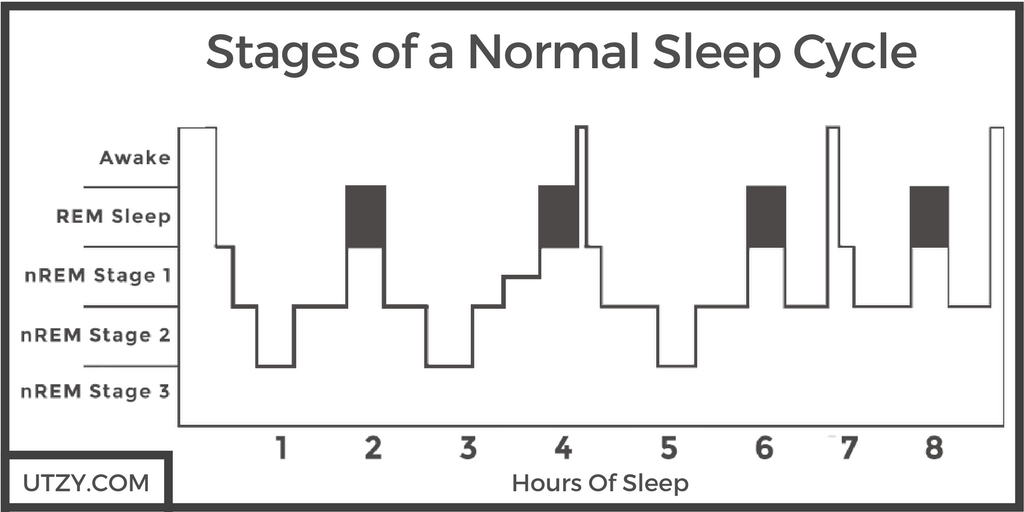
\includegraphics[width=\textwidth]{images/sleepstages.png}
\caption{Progression through the various stages of NREM and REM during nights sleep}
\label{fig: Sleep Stages}
\end{figure}

\newpage
Amount of time spent in REM sleep varies across life span 
\begin{itemize}
    \item Infants sleep 16 hours and spend half in REM stage
    \item Age one, spend around 12 hours sleeping, four hours in REM
    \item REM decreases and stabilizes by puberty at around 1.5 to 2 hours per night
\end{itemize}

During REM sleep clusters of cells in the pons and midbrain become active and spread neural excitation into the cerebral cortex. 
\begin{itemize}
    \item Neurotransmitter acetylcholine is central to this excitation, and many of these excitatory 
    REM active neurons innervating the cortex are cholinergic
    \item Results in widespread activation in cerebral cortex
    \item Produces state of neural activity like wakefulness than other stages
    \item REM-active neurons send signals to the eye muscles, triggering eye movements.
    \item Inhibition of motor output from the cortex via the spinal cord
    \item During REM, the sleeper's body is relaxed and there is little movement (except eyes). If it weren't for the inhibition of motor output, sleeper's body would jerk and move around quite a bit. 
\end{itemize}

\subsection{REM sleep and dreams}
\begin{itemize}
    \item If someone is in the REM sleep stage and are awakened, 90\% report dreaming quite vividly
    \item If awakened during NREM sleep stage, only 5\% report dreaming vividly
    \item Strong relationship between REM sleep and vivid dreaming fits with neural activity
    \item Stimulation of visual areas without visual stimulation to the eye, one may experience seeing things
\end{itemize}

\subsection{Acetylcholine and REM}
Due to cholinergic nature of cortical activation during REM, drugs that activate acetylcholine circuitry may increase vividness of dreams
\begin{itemize}
    \item Nicotine is one such drug. People who use nicotine patches report increased vividness of dreaming
        \subitem Shamans might smoke before sleeping to increase vividness of dreams
    \item Acetylcholinesterase inhibitors decrease the chemical breakdown of acetylcholine after it is released, thus prolonging its activity in the synaptic cleft. 
    \item These drugs are used in the treatment of dementia. 
\end{itemize}

\subsection{Lucid Dreaming and Dream Yoga}
Dreams are ephemeral and usually awaken with no memory at all of dreaming. \\
Lucid dreaming occurs when one becomes aware of dreaming while still asleep
\begin{itemize}
    \item One is asleep in REM, eyes closed, motor activity inhibited, and dreaming, and within the dream there is an awareness that what is happening is a dream
    \item Lucidity in dreams is valued in some cultures 
    \item Lucidity might also be regular feature of some peoples dreams
    \item You can practice by working on recalling dreams and then cultivating the intention to become aware of one's dream while dreaming
\end{itemize}

Some spiritual traditions that place high value on practice of meditation (Ex: Buddhism and Hinduism) have \textbf{dream yoga} practices
\begin{itemize}
    \item Goal: becoming regularly lucid during dream and even nondream sleep 
    \item Daily experiences influence our dream experiences
    \item In dream yoga practice, the practitioner at every moment to incline the mind toward the thoughts, feelings, and actions that honor the ethical framework of their tradition
    \item Generally, cultivation of love and compassion, for oneself and others
\end{itemize}

\section{Sleep Disorders}
\begin{itemize}
    \item \textbf{Insomnia:} difficulty with sleep, often with falling asleep
    \begin{itemize}
        \item Not a specific disorder: symptom could be associated with any number of different things. Being hyperaroused or excited during day, jet lag, noisy or uncomfortable sleep environment, stress and emotional turmoil, and sedative hypnotics even (alcohol) 
        \item Treatment: addressing condition to cause symptoms
        \item  \textbf{"Sleep Hygiene":} Optimizing conditions conducive to restful sleep: maintaining regular wake-sleep pattern, relaxing before sleep, avoiding bright light (computer screens), avoid large meals in evening, decreasing or eliminating caffeine and alcohol consumption
    \end{itemize}
    \item \textbf{Sleep Apnea:} condition where the sleeper periodically stops breathing or has abnormally shallow breathing
        \begin{itemize}
            \item Caused by obstruction or constricting of airways
            \item Sleeper wakes up from lack of air, breathing adjusts, and sleep returns
            \item However, sleep disruptions can result in fatigue and impaired performance the next day
            \item Fairly common, affects 5\% of adults
        \end{itemize}
    \item \textbf{Narcolepsy:} primary symptom, excessive daytime sleepiness, even after full night of sleep
        \begin{itemize}
            \item Nighttime cycling between NREM and REM stages is generally not normal in narcoleptics 
            \item Abnormalities related to orexin, neuropeptide involved in maintaining wakefulness
            \item Orexin derives name from \textit{orexis} (Greek), meaning appetite or desire
            \item Orexinergic neurons located in hypothalamus and send axons widely throughout the brain, to cerebral cortex and brainstem
            \item New medication to antagonisze orexin receptors to treat insomnia (different from GABA modulating drugs (benzodiazepines))
        \end{itemize}
    \item \textbf{REM behavior disorder:} impairment of motor inhibition in REM-stage sleep, resulting in sleepers acting out heir dreams. (body may flail around or move resulting in awakening)
    \item \textbf{Sleep Paralysis:} one partially awakens while in REM-stage sleep
        \begin{itemize}
            \item Person aware but unable to move the body because the neural activity of REM continues to inhibit motor output from the brain
            \item Person is likely to have vivid sensory experiences of event due to REM cortical activity
            \item See things resulting in distress or terror (because you can't move to defend yourself)
        \end{itemize}
    \item \textbf{Sleepwalking or Somnambulism:} when a person, still asleep, rises from bed and walks about
        \begin{itemize}
            \item Sometimes engaging in activities such as bathing, housecleaning, eating, and cooking or driving
            \item tends to happen while person is in deep stages of slow-wave sleep. Stages 3 and 4 of NREM
        \end{itemize}
    \item \textbf{Chronic Sleep Deprivation:} Eight hours is common "normal" human sleep time, but individuals vary widely in how much sleep they get and appear to require for optimal daytime functioning
        \begin{itemize}
            \item Most widely occurring sleep-related problem
            \item Generally, people sleep shortly after sunset and rise at sunrise
            \item Tend to sleep later due to electricity and other night activities
            \item Still awaken early the next day however resulting in consumption of coffee, tea, energy drinks and other caffeinated drinks
        \end{itemize}
\end{itemize}
Insufficient sleep impairs cognitive and motor performance. Can affect your job or studying performance and could definitely affect others. \\
Automobile accidents, plane crashes, surgical mistakes, etc. 

\section{Sleep and Learning, Memory, and Consolidation}
During sleep various restorative process operate within the body
\begin{itemize}
    \item Chemical reactions of cellular metabolism - maintaining cells in our body
    \item High reactive molecular entities are being generated
\end{itemize}

\noindent Sleep is important for \textbf{learning} and \textbf{memory}
\begin{itemize}
    \item Sleep prepares brain optimally to encode new information for storage in long-term memory
    \item \textbf{Consolidation:} helps lock the memory more securely in place after initial encoding
    \item Substantial memory consolidation occurs during sleep
    \item Repetition of activity is part of a process of strengthening the synaptic connections in these networks, solidifying these memories
\end{itemize}

Roles of REM and NREM sleep in memory storage and consolidation are actively being investigated. \\

Individuals deprived of REM-stage sleep fall into REM sleep much more rapidly on subsequent nights
\end{document}